\section{756 --- Pyramid Transition Matrix}
We are stacking blocks to form a pyramid. Each block has a color which is a one letter string.

We are allowed to place any color block $C$ on top of two adjacent blocks of colors $A$ and $B$, if and only if $ABC$ is an allowed triple.

We start with a bottom row of \fcj{bottom}, represented as a single string. We also start with a list of allowed triples \fcj{allowed}. Each allowed triple is represented as a string of length 3.

Return \fcj{true} if we can build the pyramid all the way to the top, otherwise \fcj{false}.

\paragraph{Example 1:}

\begin{flushleft}
\textbf{Input}: 

\fcj{bottom = "BCD"}, \fcj{allowed = ["BCG", "CDE", "GEA", "FFF"]}

\textbf{Output}: \fcj{true}

\textbf{Explanation}:

We can stack the pyramid like this:

\begin{figure}[H]
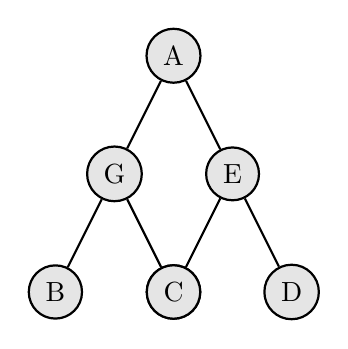
\begin{tikzpicture}
[every node/.style={draw, circle, fill=gray!20!, minimum size=5mm}, thick]
\node{A}
child{node{G} child{node{B}} child{node{C}}}
child{node{E} child{node{C}} child{node{D}}};
\end{tikzpicture}
\end{figure}

%    A
%   / \
%  G   E
% / \ / \
%B   C   D

We are allowed to place $G$ on top of $B$ and $C$ because $BCG$ is an allowed triple.  Similarly, we can place $E$ on top of $C$ and $D$, then $A$ on top of $G$ and $E$.
\end{flushleft}

 

\paragraph{Example 2:}
\begin{flushleft}


\textbf{Input}: \fcj{bottom = "AABA"}, \fcj{allowed = ["AAA", "AAB", "ABA", "ABB", "BAC"]}

\textbf{Output}: \fcj{false}

\textbf{Explanation}:

We can't stack the pyramid to the top.

Note that there could be allowed triples \fcj{(A, B, C)} and \fcj{(A, B, D)} with $C \neq D$.

\end{flushleft} 

\paragraph{Note:}

\begin{itemize}
\item \fcj{bottom} will be a string with length in range \fcj{[2, 8]}.
\item \fcj{allowed} will have length in range \fcj{[0, 200]}.
\item Letters in all strings will be chosen from the set \fcj{['A', 'B', 'C', 'D', 'E', 'F', 'G']}.

\end{itemize}

\subsection{Depth First Search}

\setcounter{lstlisting}{0}
\begin{lstlisting}[style=customc, caption={DFS}]
bool pyramidTransition( string bottom, vector<string>& allowed )
{
    unordered_map<string_view, vector<char>> dict;
    for( const auto& allow :  allowed )
    {
        string_view sv( allow );
        dict[sv.substr( 0, 2 )].push_back( sv.back() );
    }
    unordered_map<string, unsigned char> memo;
    return dfs( bottom, 0, "", dict, memo );
}
bool dfs( string start, size_t index, string next, unordered_map<string_view, vector<char>>& dict, unordered_map<string, unsigned char>& memo )
{
    if( start.size() == 1 )
    {
        return true;
    }
    auto it = memo.find( start );
    if( it != memo.end() )
    {
        return it->second != 0;
    }
    if( next.size() == start.size() - 1 )
    {
        auto res = dfs( next, 0, "", dict, memo );
        memo.emplace( next, res ? 1 : 0 );
        return res;
    }
    string_view sv( start );
    if( index <= start.size() - 2 )
    {
        auto key = sv.substr( index, 2 );
        auto it = dict.find( key );
        if( it == dict.end() )
        {
            return false;
        }
        for( auto c : it->second )
        {
            next.push_back( c );
            if( dfs( start, index + 1, next, dict, memo ) )
            {
                memo.emplace( start, 1 );
                return true;
            }
            next.pop_back();
        }
    }
    return false;
}
\end{lstlisting}